\documentclass[addpoints,answers]{exam}
\usepackage[spanish]{babel}
\usepackage[utf8]{inputenc}
\usepackage{color}
\usepackage{amsmath,amssymb,latexsym,color,graphicx}
\usepackage{multicol}
\usepackage{hyperref}
%This block of commented code translates default words to Spanish
%-------------------------------------------------------------
\pointpoints{punto}{puntos}
\bonuspointpoints{punto extra}{puntos extra}

\totalformat{Pregunta \thequestion: \totalpoints{} puntos}

\chqword{Pregunta}
\chpgword{Página}
\chpword{Página}
\chpword{Puntos}
\chbpword{Puntos extra}
\chsword{Puntos obtenidos}
\chtword{Total}

\footer{}{Página \thepage\ de \numpages}{}

%\boxedpoints
%-------------------------------------------------------------
\renewcommand{\solutiontitle}{\noindent\textbf{Solución:}\par\noindent}
\SolutionEmphasis{\color{blue}}

%Tikz
\usepackage{physics}
\usepackage{amsmath}
\usepackage{tikz}
\usepackage{mathdots}
\usepackage{yhmath}
\usepackage{cancel}
\usepackage{color}
\usepackage{siunitx}
\usepackage{array}
\usepackage{multirow}
\usepackage{amssymb}
\usepackage{gensymb}
\usepackage{tabularx}
\usepackage{extarrows}
\usepackage{booktabs}
\usetikzlibrary{fadings}
\usetikzlibrary{patterns}
\usetikzlibrary{shadows.blur}
\usetikzlibrary{shapes}


\begin{document}
%This code creates the text before the first question
%-------------------------------------------------------------------


\begin{multicols}{2}

\vspace*{0.24cm}
	
\includegraphics[scale=0.3]{FAC_INGYCIEN.jpeg}
	\begin{center}
		\textbf{Fundamentos de Economía}\\
		\textsc{Primer semestre 2022}\\
		Profesores: Sebastián Cea, Jouseline Salay, Jorge Arenas\\
		Ayudantes: Antonia Banduc, Vicente Muñoz, Roberto Wittig, Hernán Venegas
	\end{center}

\end{multicols}

\begin{center}

\sc Ayudantía 7

\end{center}


%Here, the questions begin
\begin{questions}

%First question below
\question Preguntas de concepto:
\hfill \break
\begin{parts}

\part Ubique, en un gráfico de oferta y demanda, el peso muerto producido por un impuesto.

\begin{solutionorbox}[4in]
Por definición el peso muerto es la reducción del excedente total producida por una distorsión del mercado, como lo es un impuesto. En la Figura \ref{fig:imptoPS} podemos ver una representación del fenómeno:

\begin{figure}
    \centering
    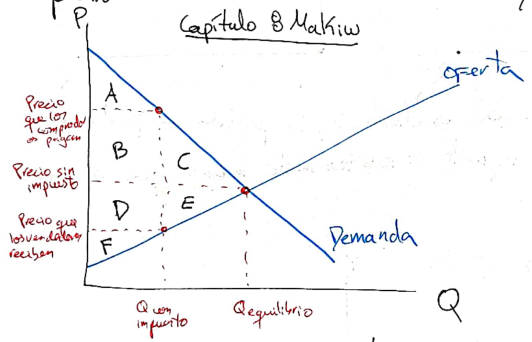
\includegraphics{Ayudantía 7/fig1.png}
    \caption{Figura 3 Capítulo 8 Mankiw}
    \label{fig:imptoPS}
\end{figure}

\end{solutionorbox}

\part Explique, con apoyo de gráficos,  cómo afecta la elasticidad de la oferta y de la demanda al peso muerto producido por un impuesto.

\part Cuando se aplican impuestos específicos a los bienes necesarios (por ejemplo, un impuesto de \$10 a la oferta de pan), son los más pobres los que siempre terminan pagando una mayor proporción del impuesto, ya que ellos se ubican en la parte baja de la curva de demanda. ¿Es correcta esa afirmación?

\end{parts}

\question Suponga el mercado de la carne de un país determinado por las siguientes funciones de oferta y demanda:

\[Q_o = -110 + 2P \hspace{0.5cm}  y \hspace{0.5cm} Q_d = 400 - P\]
\begin{parts}
\part Calcule el precio y cantidad óptimo de mercado.
\hfill \break
\part Ahora imagine que ese gobierno  luego de varios estudios cree que es conviente aplicar un subsidio de \$210, grafique y calcule que ocurriría en ese mercado.

\end{parts}

\question Imagine que el mercado del litio está dado por las siguientes funciones de oferta y demanda:
\[Q_o = 40000 + 2000P \hspace{0.5cm}  y \hspace{0.5cm} Q_d = 160000 -2000P\]
Pero ahora, para que sea posible la producción de ese litio, existe un costo marginal externo asociado a su producción $CMgE = 0.2Q$
\begin{parts}
\part Calcule precio y cantidad de equilibrio sin regulación.

\part Calcule precio y cantidad de equilibrio óptimos desde el punto de vista social. 

\part Calcule el costo social de la solución en la parte a). 

\part Estudie la opción de un impuesto para llegar al óptimo de la parte b).

\part Aplicado el nuevo impuesto, calcule los nuevos excedentes.

\end{parts}

\question El gobierno de un país quiere subsidiar con \$136 la compra de libros de economía, y para eso decide aplicar un impuesto en el mercado del alcohol. Las funciones de demanda del mercado de los libros son:

\[Q_o = 2P \hspace{0.5cm}  y \hspace{0.5cm} Q_d = 2400 -6P\]

Y las funciones del mercado del alcohol son:

\[Q_o = P \hspace{0.5cm}  y \hspace{0.5cm} Q_d = 2000 - P\]
\begin{parts}
\part ¿Cuál debe ser el monto del impuesto a aplicar sobre los alcoholes?

\end{parts}
\end{questions}


\end{document}